\documentclass[]{article}
\newcommand{\FileDepth}{../../..}
\usepackage[letterpaper, landscape, margin=0.5cm]{geometry}
\usepackage[T1]{fontenc}
\usepackage{textcomp}%Not strictly necessary, but gives \textmu command for "micro."
\usepackage{fancyhdr}
\usepackage{amsmath}
\usepackage{amssymb}
\usepackage{graphicx}
\usepackage{xcolor}
\usepackage{tikz}
\usetikzlibrary{calc}
\usepackage[shortlabels]{enumitem}
\usepackage{multicol}
\usepackage{vwcol}
\usepackage{hyperref}
\usepackage{wrapfig}
%opening
\newcommand{\SecType}{L}
\newcommand{\Week}{22}
\title{PH 211 Lecture \Week}
\author{Benjamin Bauml}
\date{Summer 2024}

\newcommand{\Purpose}{4}
\newcommand{\DefOnly}{0}

\input{\FileDepth/Formats/Assignment20240614.tex}
\usepackage[absolute]{textpos}
% This package relies on Assignment Format 2024-06-14 or later to work. It is recommended that the Purpose and DefOnly commands be given as such:
%\newcommand{\Purpose}{4}
%\newcommand{\DefOnly}{0}
% Activities need to be entered outside of the TeacherMargin and PresentSpace environments, otherwise they will be defined only locally. They can even go in the preamble.
\newenvironment{TeacherMargin}{\begin{textblock*}{10.8cm}(0.5cm,0.5cm)
\small}{\end{textblock*}
\hspace{0.1cm}}
\newenvironment{PresentSpace}{\begin{textblock*}{0.3cm}(26.85cm,9.35cm)
--
\end{textblock*}
\begin{textblock*}{15.6cm}(11.8cm,0.5cm)
\begin{Repurpose}{1}
\Large}{\end{Repurpose}
\end{textblock*}
\hspace{0.1cm}}

%\newcommand{\FBDaxes}[4][2]{
	\begin{scope}[shift={(#2)},rotate=#3]
		% x-axis
		\draw[thick,->] (-#1,0) -- (#1,0);
		\node[anchor=west] at (#1,0) {$x$};
		% y-axis
		\draw[thick,->] (0,-#1) -- (0,#1);
		\node[anchor=south] at (0,#1) {$y$};
		\coordinate (#4) at (0,0);
	\end{scope}
}
\newcommand{\FBDvectorMA}[4]{
	\begin{scope}[shift={(#1)}]
		\coordinate (#4tip) at ({#2*cos(#3)},{#2*sin(#3)});
		\draw[ultra thick,blue,->] (#1) -- (#4tip);
	\end{scope}
}
\newcommand{\FBDvectorXY}[3]{
	\begin{scope}[shift={(#1)}]
		\coordinate (#3tip) at (#2);
		\draw[ultra thick,blue,->] (0,0) -- (#3tip);
	\end{scope}
}
\newcommand{\FBDdot}[1]{
	\filldraw[black] (#1) circle (3pt);
}
\newcommand{\FBDbox}[5][1]{
	\begin{scope}[shift={(#2)},rotate=#3]
		\filldraw[color=black,fill=white,thick] ({-#1/2},{#1/2}) -- ({-#1/2},{-#1/2}) -- ({#1/2},{-#1/2}) -- ({#1/2},{#1/2}) -- cycle;
		% Left side coordinates
		\coordinate (#4ltq) at ({-#1/2},{#1/4});
		\coordinate (#4lcent) at ({-#1/2},0);
		\coordinate (#4lbq) at ({-#1/2},{-#1/4});
		% right side coordinates
		\coordinate (#4rtq) at ({#1/2},{#1/4});
		\coordinate (#4rcent) at ({#1/2},0);
		\coordinate (#4rbq) at ({#1/2},{-#1/4});
		% top coordinates
		\coordinate (#4tlq) at ({-#1/4},{#1/2});
		\coordinate (#4tcent) at (0,{#1/2});
		\coordinate (#4trq) at ({#1/4},{#1/2});
		% bottom coordinates
		\coordinate (#4blq) at ({-#1/4},{-#1/2});
		\coordinate (#4bcent) at (0,{-#1/2});
		\coordinate (#4brq) at ({#1/4},{-#1/2});
		% corners
		\coordinate (#4tl) at ({-#1/2},{#1/2});
		\coordinate (#4tr) at ({#1/2},{#1/2});
		\coordinate (#4bl) at ({-#1/2},{-#1/2});
		\coordinate (#4br) at ({#1/2},{-#1/2});
		\node at (0,0) {#5};
	\end{scope}
}
\newcommand{\MVec}[3][0]{%Creates a momentum vector of length #3 centered at #2 and rotated #1 degrees counterclockwise.
	\begin{scope}[rotate=#1,shift={(#2)}]
		\draw[->,thick] ({-#3/2},0) -- ({#3/2},0);
	\end{scope}
}
\newcommand{\MDot}[1]{%Creates a dot at #1 to represent a zero vector.
	\filldraw (#1) circle (1pt);
}
\newcommand{\MVDRows}[2][4.5]{%Creates the rows (initial, delta, final) of a momentum vector diagram. The optional argument determines the width of the table, and defaults to a good length for three columns (two objects and the total system). The non-optional argument gives a coordinate name (not displayed) to the diagram.
	\begin{scope}
		%\draw[thick] (0,5.5) -- (0,0);
		\draw[thick] (-1,4.5) -- (#1,4.5);
		\node at (-0.5,3.75) {$\vec{p}_{i}$};
		\draw[thick] (-1,3) -- (#1,3);
		\node at (-0.5,2.25) {$\Delta\vec{p}$};
		\draw[thick] (-1,1.5) -- (#1,1.5);
		\node at (-0.5,0.75) {$\vec{p}_{f}$};
		\coordinate (#2) at (0,5);
	\end{scope}
}
\newcommand{\MVDCol}[4][0.75]{%Creates a column for an object in a momentum vector diagram. The first (non-optional) argument is the coordinate name (not displayed) of the column, while the second is the displayed column header. The first argument also names the three entries down the column. The third argument anchors the column, so it should either be the coordinate name of the MVD (for the first column) or the coordinate name of the previous column. The optional argument indicates how far the center of the column should be from the previous column's edge, and defaults to 0.75.
	\begin{scope}[shift={(#4)}]
		\node at (#1,0) {#3};
		%\draw[thick] ({#1*2},0.5) -- ({#1*2},-5);
		\draw[thick] (0,0.5) -- (0,-5);
		\coordinate (#2init) at (#1,-1.25);
		\coordinate (#2delt) at (#1,-2.75);
		\coordinate (#2fin) at (#1,-4.25);
		\coordinate (#2) at ({#1*2},0);
	\end{scope}
}

\Problem{Springloaded Sled}{\SpringSled}{
You are designing a sled with a compressed spring inside, which can be released to separate the sled into two pieces of equal mass ($m/2$). You are racing the sled across level snow at speed $v$ when you trigger the separation.
%A firework is moving to the right with speed v when it explodes into two pieces with equal mass (m/2).
}
\ProblemSub{\SpringSledMomEn}{
Right after the two halves push apart, the back end of the sled is moving backward with speed $v$. What is the velocity of the other piece? How much kinetic energy did the system gain?
%Right after the explosion, the first piece is moving backward with speed v.
%What is the velocity of the other piece?
%How much kinetic energy did the system gain?
}
\ProblemFig{\SpringSledFig}{
\centering
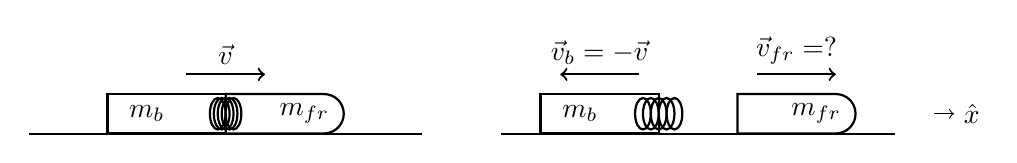
\begin{tikzpicture}
	\begin{scope}[rotate=0,shift={(-3,0)}]
		\draw[thick,->] (-0.5,0.5) -- (0.5,0.5);
		\node[anchor=south] at (0,0.5) {$\vec{v}$};
		\begin{scope}
			\draw[thick] (-1.5,0.25) rectangle (0,-0.25);
			\node at (-1,0) {$m_{b}$};
		\end{scope}
		\begin{scope}
			\draw[thick] (0,0.25) -- (1.25,0.25) arc (90:-90:0.25) -- (0,-0.25) -- cycle;
			\node at (1,0) {$m_{fr}$};
		\end{scope}
		\begin{scope}[yscale=2]
			\newcommand{\Comp}{0.05}
			\draw[thick] ({-\Comp*2},0) circle (0.1);
			\draw[thick] (-\Comp,0) circle (0.1);
			\draw[thick] (0,0) circle (0.1);
			\draw[thick] (\Comp,0) circle (0.1);
			\draw[thick] ({\Comp*2},0) circle (0.1);
		\end{scope}
		\draw[thick] (-2.5,-0.26) -- (2.5,-0.26);
	\end{scope}
	\begin{scope}[rotate=0,shift={(3,0)}]
		\begin{scope}[shift={(-0.5,0)}]
			\draw[thick,->] (-0.25,0.5) -- (-1.25,0.5);
			\node[anchor=south] at (-0.75,0.5) {$\vec{v}_{b}=-\vec{v}$};
			\draw[thick] (-1.5,0.25) rectangle (0,-0.25);
			\node at (-1,0) {$m_{b}$};
		\end{scope}
		\begin{scope}[shift={(0.5,0)}]
			\draw[thick,->] (0.25,0.5) -- (1.25,0.5);
			\node[anchor=south] at (0.75,0.5) {$\vec{v}_{fr}=$?};
			\draw[thick] (0,0.25) -- (1.25,0.25) arc (90:-90:0.25) -- (0,-0.25) -- cycle;
			\node at (1,0) {$m_{fr}$};
		\end{scope}
		\begin{scope}[yscale=2,shift={(-0.5,0)}]
			\newcommand{\Comp}{0.1}
			\draw[thick] ({-\Comp*2},0) circle (0.1);
			\draw[thick] (-\Comp,0) circle (0.1);
			\draw[thick] (0,0) circle (0.1);
			\draw[thick] (\Comp,0) circle (0.1);
			\draw[thick] ({\Comp*2},0) circle (0.1);
		\end{scope}
		\draw[thick] (-2.5,-0.26) -- (2.5,-0.26);
	\end{scope}
	\begin{scope}[shift={(6,0)}]
		\draw[->] (0,0) -- (0.25,0);
		\node[anchor=west] at (0.25,0) {$\hat{x}$};
	\end{scope}
\end{tikzpicture}
}
\Solution{\SpringSledSol}{
	
When setting up a motion vector diagram for this problem, I know the initial momentum of the combined sled system, and I know both parts of the sled have half of this momentum. I also know that the final momentum of the back half is reversed, and the total momentum of the system is unchanged, so I can infer the rest of the table from there.
\begin{figure}[h]
	\centering
	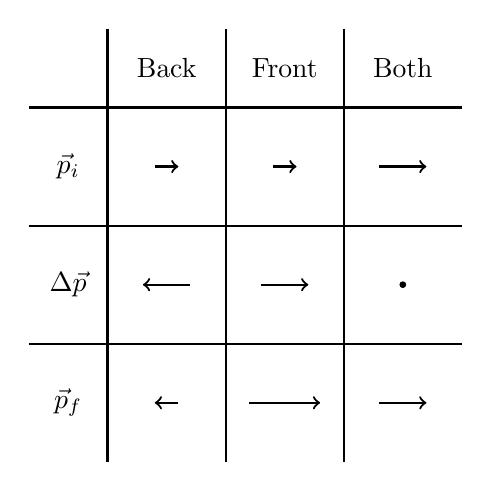
\begin{tikzpicture}
		\MVDRows{MVD}
		\MVDCol{mass}{Back}{MVD}{0.75}
		\MVec{massinit}{0.3}
		\MVec[180]{massdelt}{0.6}
		\MVec[180]{massfin}{0.3}
		\MVDCol{Mass}{Front}{mass}{0.75}
		\MVec{Massinit}{0.3}
		\MVec{Massdelt}{0.6}
		\MVec{Massfin}{0.9}
		\MVDCol{sys}{Both}{Mass}{0.75}
		\MVec{sysinit}{0.6}
		\MDot{sysdelt}
		\MVec{sysfin}{0.6}
	\end{tikzpicture}
\end{figure}

The initial momentum of the system is $mv\hat{x}$, and the final momentum is $(\frac{m}{2}v_{fr}-\frac{m}{2}v)\hat{x}$. Since the momentum is conserved (no friction, and the normal force and gravitational force are in balance, so no other net impulse), we know that
\begin{align*}
	mv\hat{x} & = \left(\frac{m}{2}v_{fr}-\frac{m}{2}v\right)\hat{x} \\
	mv & = \frac{m}{2}v_{fr}-\frac{m}{2}v \\
	2v & = v_{fr} - v \\
	v_{fr} & = 3v.
\end{align*}
The front half of the sled gets launched forward at triple its original speed!

As for kinetic energy, the system started with $K_{i} = \frac{1}{2}mv^{2}$, and now it has
\[
K_{f} = \frac{1}{2}\frac{m}{2}v^{2} + \frac{1}{2}\frac{m}{2}(3v)^{2} = \frac{5}{2}mv^{2},
\]
therefore the change in kinetic energy is
\[
\Delta K = K_{f}-K_{i} = 2mv^{2}.
\]

This came from the spring. If the spring constant is $k$ and the spring was compressed by a length $\Delta x$, then we have
\begin{align*}
\frac{1}{2}k\Delta x^{2} & = 2mv^{2} \\
k\Delta x^{2} & = 4mv^{2}.
\end{align*}
This has some interesting design implications. For example, say each half of our sled is 100 kg (say that accounts for the machinery and the load of a single passenger on each half) and its initial speed was a lazy 1 m/s. That would mean the spring has to store 400 J of energy. If $\Delta x = 0.5$ m (which may be too much of a compression for a reasonable use of Hooke's law), then $k=3200$ N/m (or 32 N/cm), which is a pretty stiff spring. If we cannot get a spring this stiff, then we need more compression, but if we cannot obtain a spring that compresses far enough without permanently deforming, then we need it stiffer. The key will be finding the perfect middle ground. It is also worth considering whether having only a single spring is the best option.
}
%\input{\FileDepth/Activities/Activity_Two/Activity_Two.tex}

\begin{document}
\begin{TeacherMargin}

\end{TeacherMargin}
\begin{PresentSpace}
\begin{center}
	\huge Lecture \Week: Inelastic and Superelastic Collisions
\end{center}
\vspace{0.5cm}
\underline{Announcements}
\begin{itemize}
	\item End-of-Term Individual Meetings Open
	\begin{itemize}
		\item 30 minute time slots to discuss anything before the final ungrading.
		\begin{itemize}
			\item Wednesday: 10:00 -- 11:30 a.m., 3:30 -- 5:00 p.m.
			\item Thursday: 10:00 a.m. -- 2:00 p.m., 4:00 p.m. -- 5:30 p.m.
			\item Friday: 11:00 -- 11:30 a.m., 3:30 -- 5:00 p.m.
		\end{itemize}
		\item Must be booked at least 5 hours in advance (recommended to book far sooner).
		\item Only 21 slots; ask me if you need to meet and nothing is available.
	\end{itemize}
\end{itemize}
\end{PresentSpace}
\newpage
\begin{TeacherMargin}
\noindent\textbf{Case 1} \\
To set up a momentum vector diagram for case 1, I began with entering the initial momenta for the two cars, which told me the initial momentum for the whole system. I also assumed that momentum was conserved (by the reasoning listed in L20-1), which allowed me to fill in the 1 \& 2 column. Since the cars get tangled at the end, I know they have the same speed, and I know Car 2 is twice as big as Car 1, so it should have twice the momentum (which means it will have two thirds of the momentum of the whole system). This allowed me to fill in the rest of the final momentum row. The last two entries in the change in momentum row are now determined by the other entries in their columns.
\begin{center}
	\Large
	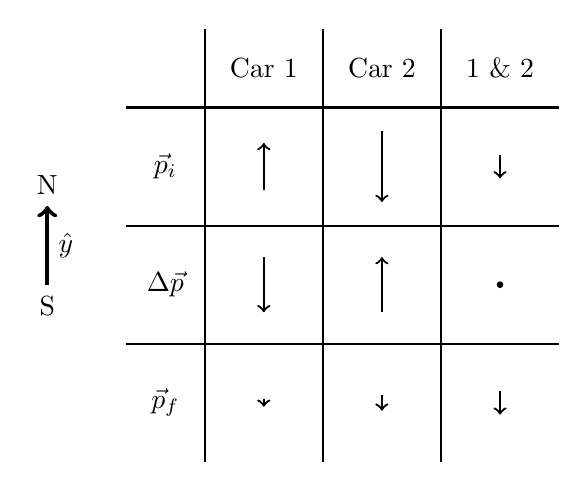
\begin{tikzpicture}
		\draw[ultra thick,->] (0,0) node[anchor=north] {S} -- (0,0.5) node[anchor=west] {$\hat{y}$} -- (0,1) node[anchor=south] {N};
		\begin{scope}[shift={(2,-2.25)}]
			\MVDRows{Caseone}
			\MVDCol{Carone}{Car 1}{Caseone}
			\MVec[90]{Caroneinit}{0.6}
			\MVec[270]{Caronedelt}{0.7}
			\MVec[270]{Caronefin}{0.1}
			\MVDCol{Cartwo}{Car 2}{Carone}
			\MVec[270]{Cartwoinit}{0.9}
			\MVec[90]{Cartwodelt}{0.7}
			\MVec[270]{Cartwofin}{0.2}
			\MVDCol{Cars}{1 \& 2}{Cartwo}
			\MVec[270]{Carsinit}{0.3}
			\MDot{Carsdelt}
			\MVec[270]{Carsfin}{0.3}
		\end{scope}
	\end{tikzpicture}
\end{center}
Already, I know that my cars should go south after the collision. Let us calculate the velocity.
\begin{align*}
	m_{1} & = 100\text{ kg} & m_{2} & = 200\text{ kg} & m_{f} & = m_{1}+m_{2} \\
	\vec{v}_{1} & = (4\text{ m/s})\hat{y} & \vec{v}_{2} & = -(3\text{ m/s})\hat{y} & \vec{v}_{f} & = v_{f}\hat{y} = ?
\end{align*}
\begin{align*}
	\vec{p}_{i} & = m_{1}\vec{v}_{1} + m_{2}\vec{v}_{2} = (m_{1}v_{1}-m_{2}v_{2})\hat{y} \\
	\vec{p}_{f} & = (m_{1} + m_{2})\vec{v}_{f} = (m_{1}+m_{2})v_{f}\hat{y}
\end{align*}
\begin{align*}
	\vec{p}_{i} & = \vec{p}_{f} & v_{f} & = \frac{m_{1}v_{1}-m_{2}v_{2}}{m_{1}+m_{2}} \\
	m_{1}v_{1} - m_{2}v_{2} & = (m_{1}+m_{2})v_{f} &  & = \frac{(100\text{ kg})(4\text{ m/s})-(200\text{ kg})(3\text{ m/s})}{100\text{ kg}+200\text{ kg}} \\
	& & & = \frac{400-600}{300}\text{ m/s} = -\frac{2}{3}\text{ m/s}
\end{align*}
\begin{align*}
	K_{i} & = \frac{1}{2}m_{1}v_{1}^{2} + \frac{1}{2}m_{2}v_{2}^{2} \\
	& = \frac{1}{2}(100\text{ kg})(4\text{ m/s})^{2} + \frac{1}{2}(200\text{ kg})(3\text{ m/s})^{2} = 800\text{ J} + 900\text{ J} = 1700\text{ J} \\
	K_{f} & = \frac{1}{2}(m_{1}+m_{2})v_{f}^{2} = \frac{1}{2}(300\text{ kg})\left(\frac{2}{3}\text{ m/s}\right)^{2} = \frac{200}{3}\text{ J} \approx 66.7\text{ J}
\end{align*}
A lot of energy is lost to heat and deformation of metal.
\end{TeacherMargin}
\begin{PresentSpace}
\vspace{-10pt}
\section*{L\Week-1: Bumper Cars}
\vspace{-10pt}
\begin{itemize}
	\item Two bumper cars collide with each other and get tangled together.
	\item Car 1 ($m_{1}$) moves north at $v_{1}$. Car 2 ($m_{2}$) moves south at $v_{2}$.
\end{itemize}
\begin{multicols}{2}
	\begin{itemize}
		\item Case 1
		\begin{itemize}
			\large
			\item Car 1 (100 kg) moves north at 4 m/s.
			\item Car 2 (200 kg) moves south at 3 m/s.
			\item Find the final velocity of the cars.
			\item Determine the initial and final kinetic energies of the cars.
			\item Compare the total kinetic energy before and after the collision.
		\end{itemize}
		\item Case 2
		\begin{itemize}
			\large
			\item Car 1 (100 kg) moves north at 4 m/s.
			\item Car 2 (200 kg) moves south.
			\item Find the initial velocity of Car 2 assuming they both end at rest.
			\item Determine the initial and final kinetic energies of the cars.
			\item Compare the total kinetic energy before and after the collision.
		\end{itemize}
	\end{itemize}
\end{multicols}
\end{PresentSpace}
\newpage
\begin{TeacherMargin}
\noindent\textbf{Case 2} \\
To set up a momentum vector diagram for case 2, I began with entering the initial momentum for Car 1, along with the entire final momentum row (which is all zero). for the two cars, which told me the initial momentum for the whole system. I also assumed that momentum was conserved (by the reasoning listed in L20-1), which allowed me to fill in the 1 \& 2 column with more zeros. The zero final momentum in the Car 1 column let me fill in the first car's change in momentum, then the zeros in the 1 \& 2 column helped me to fill in the momenta for Car 2.
\begin{center}
	\Large
	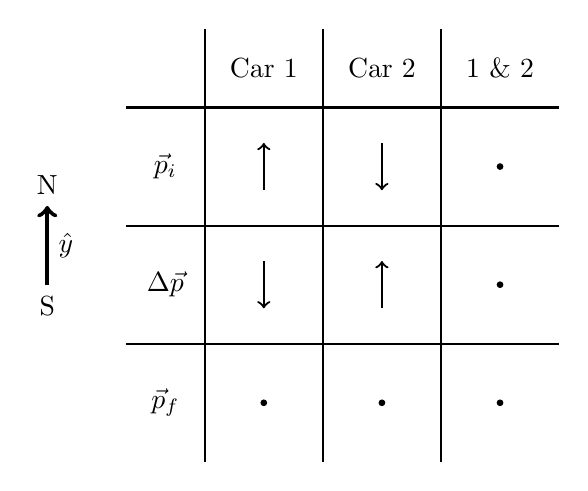
\begin{tikzpicture}
		\draw[ultra thick,->] (0,0) node[anchor=north] {S} -- (0,0.5) node[anchor=west] {$\hat{y}$} -- (0,1) node[anchor=south] {N};
		\begin{scope}[shift={(2,-2.25)}]
			\MVDRows{Caseone}
			\MVDCol{Carone}{Car 1}{Caseone}
			\MVec[90]{Caroneinit}{0.6}
			\MVec[270]{Caronedelt}{0.6}
			\MDot{Caronefin}
			\MVDCol{Cartwo}{Car 2}{Carone}
			\MVec[270]{Cartwoinit}{0.6}
			\MVec[90]{Cartwodelt}{0.6}
			\MDot{Cartwofin}
			\MVDCol{Cars}{1 \& 2}{Cartwo}
			\MDot{Carsinit}
			\MDot{Carsdelt}
			\MDot{Carsfin}
		\end{scope}
	\end{tikzpicture}
\end{center}
Already, I know that the second car must have equal and opposite initial momentum to the first car.
\begin{align*}
	m_{1} & = 100\text{ kg} & m_{2} & = 200\text{ kg} & m_{f} & = m_{1}+m_{2} \\
	\vec{v}_{1} & = (4\text{ m/s})\hat{y} & \vec{v}_{2} & = -v_{2}\hat{y} = ? & \vec{v}_{f} & = \vec{0}
\end{align*}
\begin{align*}
	\vec{p}_{i} & = m_{1}\vec{v}_{1} + m_{2}\vec{v}_{2} = (m_{1}v_{1}-m_{2}v_{2})\hat{y} \\
	\vec{p}_{f} & = (m_{1} + m_{2})\vec{v}_{f} = \vec{0}
\end{align*}
\begin{align*}
	\vec{p}_{i} & = \vec{p}_{f} & v_{2} & = \frac{m_{1}}{m_{2}}v_{1} \\
	m_{1}v_{1} - m_{2}v_{2} & = 0 &  & = \frac{1}{2}v_{1} \\
	& & & = 2\text{ m/s}
\end{align*}
Car 2 was going 2 m/s (to the south). They both end at rest, so $K_{f}=0$ J.
\begin{align*}
	K_{i} & = \frac{1}{2}m_{1}v_{1}^{2} + \frac{1}{2}m_{2}v_{2}^{2} \\
	& = \frac{1}{2}(100\text{ kg})(4\text{ m/s})^{2} + \frac{1}{2}(200\text{ kg})(2\text{ m/s})^{2} = 800\text{ J} + 400\text{ J} = 1200\text{ J}
\end{align*}
All of the energy was lost to heat and deformation of metal.
\end{TeacherMargin}
\begin{PresentSpace}
\vspace{-10pt}
\section*{L\Week-1: Bumper Cars}
\vspace{-10pt}
\begin{itemize}
	\item Two bumper cars collide with each other and get tangled together.
	\item Car 1 ($m_{1}$) moves north at $v_{1}$. Car 2 ($m_{2}$) moves south at $v_{2}$.
\end{itemize}
\begin{multicols}{2}
	\begin{itemize}
		\item Case 1
		\begin{itemize}
			\large
			\item Car 1 (100 kg) moves north at 4 m/s.
			\item Car 2 (200 kg) moves south at 3 m/s.
			\item Find the final velocity of the cars.
			\item Determine the initial and final kinetic energies of the cars.
			\item Compare the total kinetic energy before and after the collision.
		\end{itemize}
		\item Case 2
		\begin{itemize}
			\large
			\item Car 1 (100 kg) moves north at 4 m/s.
			\item Car 2 (200 kg) moves south.
			\item Find the initial velocity of Car 2 assuming they both end at rest.
			\item Determine the initial and final kinetic energies of the cars.
			\item Compare the total kinetic energy before and after the collision.
		\end{itemize}
	\end{itemize}
\end{multicols}
\end{PresentSpace}
\newpage
\setcounter{ActNumber}{1}
\begin{TeacherMargin}
\begin{multicols}{2}
\SpringSledSol
\end{multicols}
\end{TeacherMargin}
\begin{PresentSpace}
\SpringSled
\SpringSledMomEn
\SpringSledFig
\end{PresentSpace}
\newpage
\begin{TeacherMargin}
	
\end{TeacherMargin}
\begin{PresentSpace}
\section*{Main Ideas}
\begin{itemize}
	\item When kinetic energy is lost in a collision, the collision is \textit{inelastic}.
	\begin{itemize}
		\item A collision in which the objects stick together and move with the same velocity is \textit{perfectly inelastic}.
	\end{itemize}
	\item When kinetic energy increases in a collision, the collision is \textit{superelastic}.
\end{itemize}
\end{PresentSpace}
\end{document}